\chapter{Исследовательская часть}

В данном разделе будут приведены примеры работы программы, и будет проведен сравнительный анализ реализованных алгоритмов сортировки по затраченному процессорному времени.

\section{Технические характеристики}

Тестирование проводилось на устройстве со следующими техническими характеристиками:

\begin{itemize}
	\item операционная система: Ubuntu 20.04.1 Linux x86\_64 \cite{linux};
	\item память : 8 GiB;
	\item процессор: AMD® Ryzen™ 3 3200u \cite{amd}.
\end{itemize}

Тестирование проводилось на ноутбуке, включенном в сеть электропитания. Во время тестирования ноутбук был нагружен только встроенными приложениями окружения, а также непосредственно системой тестирования.

\clearpage

\section{Демонстрация работы программы}

На рисунке \ref{img:example} приведен пример работы программы.

\begin{figure}[H]
	\begin{center}
		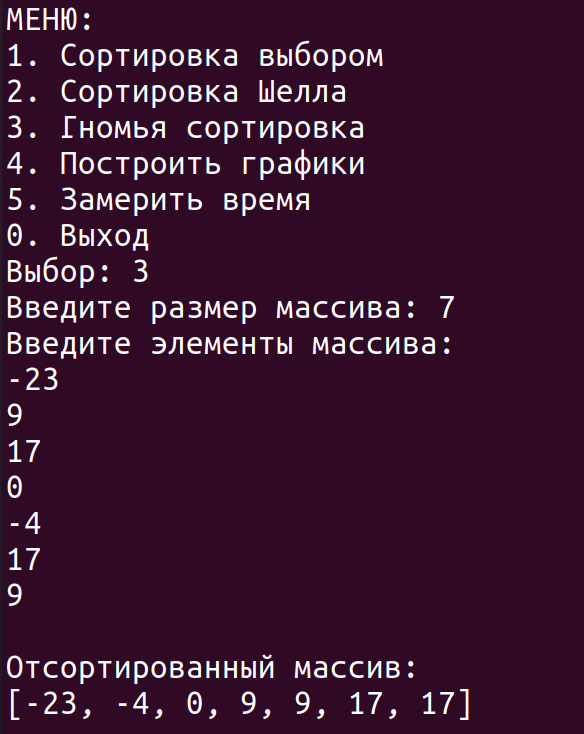
\includegraphics[scale=0.4]{img/example.png}
	\end{center}
	\captionsetup{justification=centering}
	\caption{Пример работы программы}
	\label{img:example}
\end{figure}

\section{Время выполнения алгоритмов}

Функция process\_time из библиотеки time ЯП Python возвращает сумму системного и пользовательского процессорного времени в секундах - значение типа float.

Для замера времени:
\begin{itemize}
	\item получить значение времени до начала сортировки, затем после её окончания. Чтобы получить результат, необходимо вычесть из второго значения первое;
	\item первый шаг необходимо повторить iters раз, суммируя полученные значения, а затем усреднить результат.
\end{itemize}

Результаты замеров времени работы алгоритмов в миллисекундах приведены в таблицах \ref{tbl:best}, \ref{tbl:worst}, \ref{tbl:random}.

\begin{table}[h]
	\begin{center}
		\begin{threeparttable}
		\captionsetup{justification=raggedleft,singlelinecheck=off}
		\caption{На входе отсортированный массив}
		\label{tbl:best}
		\begin{tabular}{|c|c|c|c|}
			\hline
			Размер & Выбором & Шелла & Гномья \\
			\hline
  			100 & 0.1872 & 0.4463 & 0.0107 \\ 
 			\hline
  			200 & 0.6648 & 1.5769 & 0.0208 \\ 
 			\hline
  			300 & 1.7652 & 4.2090 & 0.0315 \\ 
 			\hline
  			400 & 2.9205 & 6.5499 & 0.0415 \\ 
 			\hline
  			500 & 4.7658 & 9.9785 & 0.0527 \\ 
 			\hline
  			600 & 6.9592 & 17.5923 & 0.0610 \\ 
 			\hline
  			700 & 9.5135 & 23.0703 & 0.0695 \\ 
 			\hline
  			800 & 12.3131 & 26.6032 & 0.0836 \\ 
 			\hline
  			900 & 15.3724 & 32.2987 & 0.0905 \\ 
 			\hline
 			1000 & 18.7373 & 39.5696 & 0.0996 \\ 
 			\hline
		\end{tabular}
		\end{threeparttable}
    \end{center}
\end{table}

\begin{table}[h]
	\begin{center}
		\begin{threeparttable}
		\captionsetup{justification=raggedleft,singlelinecheck=off}
		\caption{На входе отсортированный в обратном порядке массив}
		\label{tbl:worst}
		\begin{tabular}{|c|c|c|c|}
			\hline
			Размер & Выбором & Шелла & Гномья \\
			\hline
  			100 & 0.2276 & 0.4635 & 1.4289 \\ 
 			\hline
  			200 & 0.8215 & 1.6202 & 5.4438 \\ 
 			\hline
  			300 & 2.1278 & 4.2667 & 12.9537 \\ 
 			\hline
  			400 & 3.5504 & 6.6461 & 23.6392 \\ 
 			\hline
  			500 & 5.6489 & 10.0919 & 37.7889 \\ 
 			\hline
  			600 & 8.3033 & 17.7157 & 55.5283 \\ 
 			\hline
  			700 & 11.2540 & 23.2613 & 77.0185 \\ 
			\hline
  			800 & 14.8231 & 26.7550 & 102.4330 \\ 
 			\hline
  			900 & 18.7517 & 33.3306 & 129.7009 \\ 
 			\hline
 			1000 & 23.4290 & 41.0557 & 161.5674 \\ 
 			\hline
		\end{tabular}
		\end{threeparttable}
    \end{center}
\end{table}

\clearpage

\begin{table}[h]
	\begin{center}
		\begin{threeparttable}
		\captionsetup{justification=raggedleft,singlelinecheck=off}
		\caption{На входе случайный массив}
		\label{tbl:random}
		\begin{tabular}{|c|c|c|c|}
			\hline
			Размер & Выбором & Шелла & Гномья \\
			\hline
  			100 & 0.2079 & 0.4813 & 0.7389 \\ 
 			\hline
  			200 & 0.7309 & 1.7043 & 3.0184 \\ 
 			\hline
  			300 & 1.8340 & 4.3971 & 6.5836 \\ 
 			\hline
  			400 & 3.1248 & 6.9417 & 12.2080 \\ 
 			\hline
  			500 & 4.9933 & 10.3987 & 19.7805 \\ 
 			\hline
  			600 & 7.3488 & 18.3833 & 29.6323 \\ 
 			\hline
  			700 & 10.0685 & 23.9719 & 40.9918 \\ 
 			\hline
  			800 & 13.3175 & 27.9766 & 54.7456 \\ 
 			\hline
  			900 & 17.1284 & 34.7869 & 70.0897 \\ 
 			\hline
 			1000 & 20.7750 & 41.5146 & 87.0879 \\ 
 			\hline
		\end{tabular}
		\end{threeparttable}
    \end{center}
\end{table}

На рисунках \ref{img:best-type}, \ref{img:worst-type}, \ref{img:random-type} приведены графические результаты замеров времени работы сортировок от длины входного массива в трех случаях: на входе отсортированный массив, отсортированный в обратном порядке и массив, заполненный случайным образом.

\begin{figure}[H]
	\begin{center}
		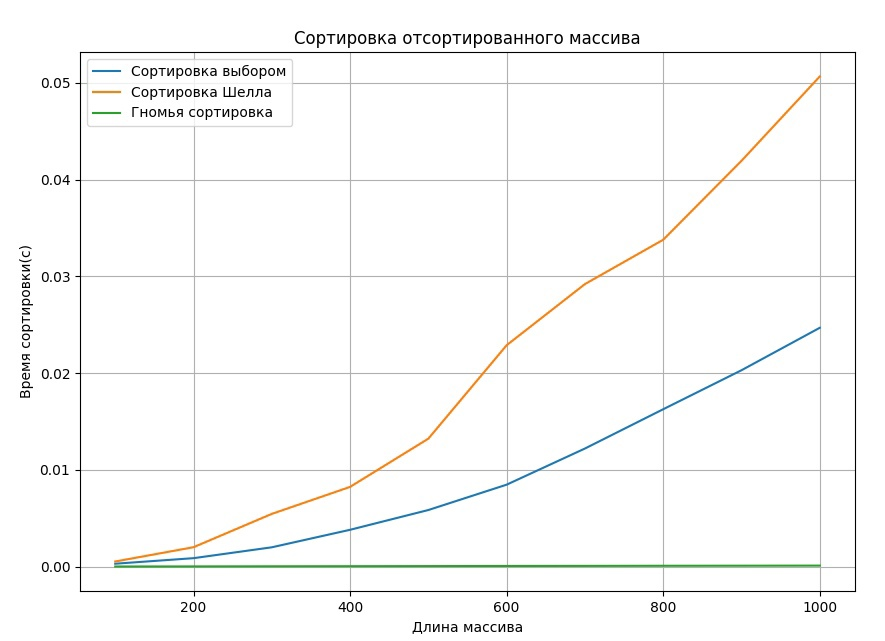
\includegraphics[scale=0.4]{img/best-type.jpg}
	\end{center}
	\captionsetup{justification=centering}
	\caption{На входе отсортированный массив}
	\label{img:best-type}
\end{figure}

\begin{figure}[H]
	\begin{center}
		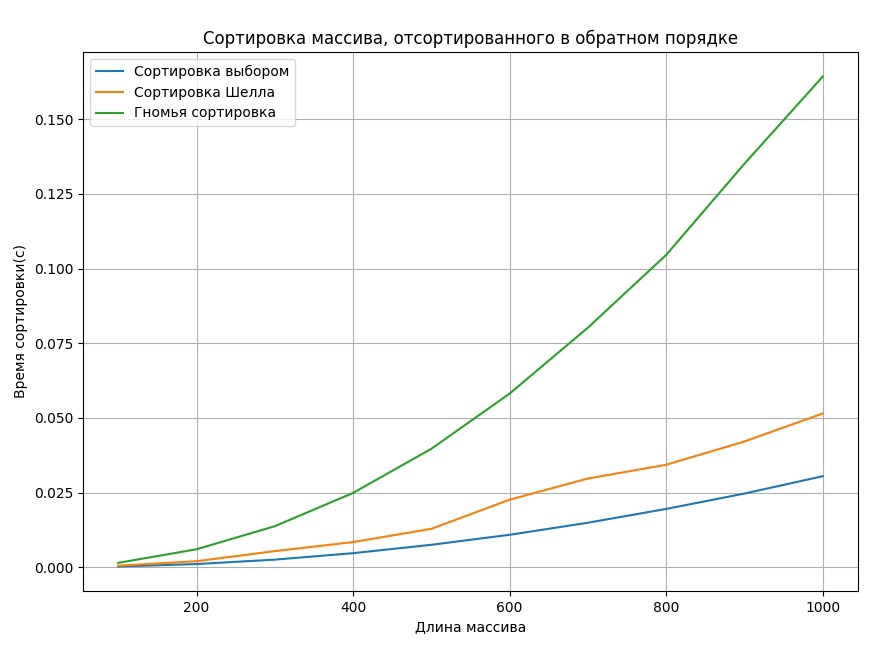
\includegraphics[scale=0.4]{img/worst-type.jpg}
	\end{center}
	\captionsetup{justification=centering}
	\caption{На входе отсортированный в обратном порядке массив}
	\label{img:worst-type}
\end{figure}

\begin{figure}[H]
	\begin{center}
		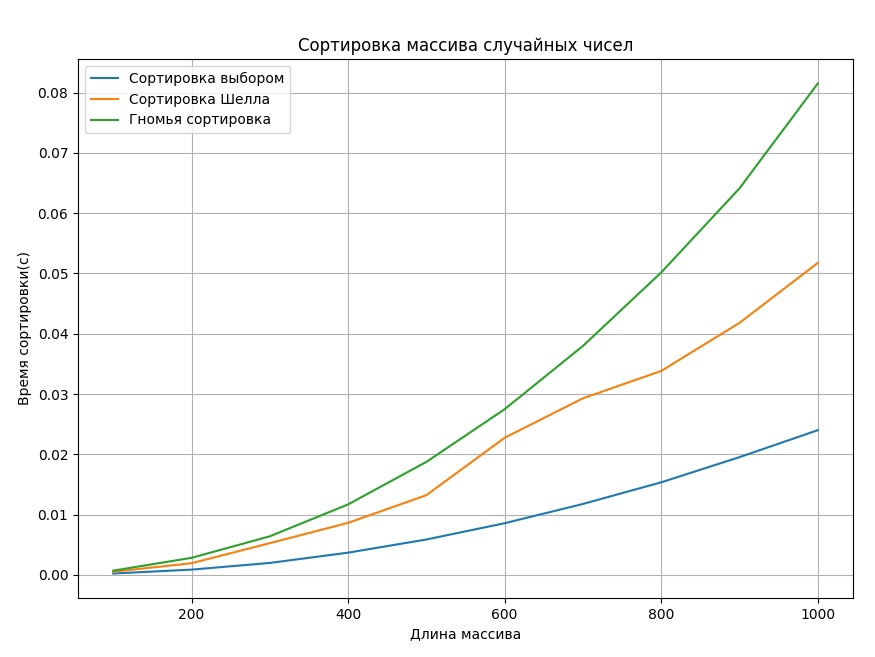
\includegraphics[scale=0.4]{img/random-type.jpg}
	\end{center}
	\captionsetup{justification=centering}
	\caption{На входе заполненный случайно массив}
	\label{img:random-type}
\end{figure}

\section*{Вывод}

Сортировка выбором работает быстрее при сортировке случайно заполненного массива и обратно отсортированного массива. Гномья сортировка в этих случаях работает дольше всех. При этом в случае отсортированного массива гномья сортировка оказывается самой быстрой, самой медленной оказывается сортировка Шелла.